\documentclass[11pt,a4paper]{article}

% =========================================================================
% PACKAGES
% =========================================================================
\usepackage[utf8]{inputenc}
\usepackage[margin=1.8cm,top=1.8cm,bottom=1.8cm]{geometry}
\usepackage{graphicx}
\usepackage{booktabs}
\usepackage{tabularx}
\usepackage{titlesec}
\usepackage{fancyhdr}
\usepackage{subcaption}
\usepackage{float}
\usepackage{hyperref}
\usepackage{amsmath}

\hypersetup{
    colorlinks=true,
    linkcolor=black,
    citecolor=black,
    urlcolor=black
}

\titleformat{\section}
  {\normalfont\Large\bfseries}{\thesection}{1em}{}[{\titlerule[0.8pt]}]

\titleformat{\subsection}
  {\normalfont\large\bfseries}{\thesubsection}{1em}{}

\setlength{\parindent}{0pt}
\setlength{\parskip}{6pt}

\pagestyle{fancy}
\fancyhf{}
\lhead{\footnotesize IIITDM Kurnool --- Department of ECE | EPM Laboratory}
\rhead{\footnotesize Divyansh Rawat (124EC0030)}
\cfoot{\thepage}
\renewcommand{\headrulewidth}{0.4pt}
\renewcommand{\footrulewidth}{0.4pt}

\begin{document}

% =========================================================================
% PAGE 1: OFFICIAL IIITDM KURNOOL CERTIFICATE & COVER PAGE
% =========================================================================
\thispagestyle{empty}

\begin{center}
    
\includegraphics[width=2.8cm]{iiitdm_logo.png}\\[8pt]
    {\Large \textbf{INDIAN INSTITUTE OF INFORMATION TECHNOLOGY}}\\[2pt]
    {\Large \textbf{DESIGN AND MANUFACTURING KURNOOL}}\\[4pt]
    {\small (An Institute of National Importance under Ministry of Education, Govt. of India)}\\[2pt]
    {\footnotesize Jagannathagattu, Dinnedevarapadu, Kurnool -- 518008, Andhra Pradesh}\\[20pt]
\end{center}

\begin{flushright}
    \textbf{Reg. No. : 124EC0030}
\end{flushright}

\vspace{4mm}

\begin{center}
    \fbox{\Large \textbf{\quad CERTIFICATE \quad}}
\end{center}

\vspace{6mm}

\begin{center}
    \normalsize
    Certified that this is the bonafide record of practical work done\\[12pt]
    by \textbf{Mr. Divyansh Rawat (Reg. No: 124EC0030)}\\[12pt]
    of the \textbf{Department of Electronics and Communication Engineering}\\[12pt]
    in the \textbf{Electronic Prototyping and Manufacturing (EPM) Laboratory}\\[12pt]
    for the Mid Semester Practical Examination on\\[4pt]
    \textbf{School/College Quiz Buzzer (8 Players) with 5V Regulated Power Supply}\\[12pt]
    during the academic year 2026 -- 2027.\\[12pt]
    \textbf{Course Faculty:} Dr. Eswaramoorthy K V
\end{center}

\vspace{6mm}

\begin{table}[H]
\centering
\small
\renewcommand{\arraystretch}{1.3}
\begin{tabular}{|l|l|}
\hline
\textbf{Student Name:} & Divyansh Rawat (Roll No: 124EC0030) \\ \hline
\textbf{Course Faculty / Examiner:} & Dr. Eswaramoorthy K V \\ \hline
\textbf{Date of Examination:} & 11-11-2026 \\ \hline
\textbf{Examination Topic:} & School/College Quiz Buzzer (8 Players, EFY Reference) \\ \hline
\textbf{Board Specification:} & Double-Layer FR4 ($200 \times 160$\,mm), Solid GND Plane \\ \hline
\textbf{Verification Status:} & \textbf{0 ERC Errors, 0 ERC Warnings, 0 DRC Violations, 100\% Netlist Parity} \\ \hline
\end{tabular}
\end{table}

\vfill

\noindent
\begin{tabularx}{\textwidth}{X r}
\textbf{Signature of Head of the Department} & \textbf{Signature of Faculty} \\[25pt]
 & \textbf{Dr. Eswaramoorthy K V} \\[4pt]
 & \textit{Associate Professor, Dept. of ECE} \\[6pt]
Date: \rule{4cm}{0.4pt} & Date: \rule{4cm}{0.4pt} \\
\end{tabularx}

\clearpage

% =========================================================================
% PAGE 2: CIRCUIT SPECIFICATION & THEORETICAL ANALYSIS
% =========================================================================
\section{Circuit Architecture \& Functional Description}

\textbf{Source Reference:} Electronics For You (EFY March 10, 2017) --- \textit{School/College Quiz Buzzer (8 Players) with 5V Regulated Power Supply}.

\subsection{Architectural Blocks}
The circuit consists of four tightly synchronized functional stages designed for high-reliability competitive buzzer lockout:

\begin{enumerate}
    \item \textbf{AC Mains Regulated Power Supply:} Steps down $230\,\text{V AC}$ mains to $7.5\,\text{V AC}$ using step-down transformer $X_1$ ($230\,\text{V} \to 7.5\,\text{V}$, $500\,\text{mA}$). The AC is converted to pulsating DC via a $1\,\text{A}$ bridge rectifier ($BR_1$), smoothed by a $1000\,\mu\text{F}/25\,\text{V}$ electrolytic reservoir capacitor ($C_1$), and linearly regulated to ultra-stable $+5\,\text{V DC}$ using an LM7805 three-terminal regulator ($IC_1$) bypassed with a $0.1\,\mu\text{F}$ ceramic capacitor ($C_2$).
    \item \textbf{Player Input Interface:} 8 independent tactile push switches ($S_1$--$S_8$) connected to $+5\,\text{V}$. Each input is pulled down to GND through a dedicated $1.2\,\text{k}\Omega$ resistor ($R_1$--$R_8$) to guarantee unambiguous logic-low states until a contestant presses a button. An 8-pin remote connector ($J_2$) enables extended corded podium switches.
    \item \textbf{Octal Transparent Latch \& Hardware Lockout:} Built around the 74LS373 octal transparent latch ($IC_2$). The latch enable pin ($\text{LE}$, pin 11) is normally held at logic high through pull-up resistor $R_{11}$ ($56\,\text{k}\Omega$), rendering the latch transparent ($Q = D$).
    \item \textbf{Diode OR-ing \& Annunciator Stage:} 8 switching diodes ($D_1$--$D_8$, 1N4148) form a high-speed wired-OR bus. When any output ($Q_0$--$Q_7$) transitions to logic high, the cathode bus instantly pulls up, driving lockout transistor $T_2$ (BC548) into saturation via base resistor $R_{10}$ ($1\,\text{k}\Omega$). $T_2$ grounds the $\text{LE}$ pin, latching the state of all outputs and locking out all subsequent contestant presses. Simultaneously, buzzer driver transistor $T_1$ activates piezo sounder $PZ_1$. The active output fires its corresponding Silicon Controlled Rectifier ($SCR_1$--$SCR_8$, TYN612), latching on the contestant's indicator lamp ($BL_1$--$BL_8$).
\end{enumerate}

\begin{figure}[H]
    \centering
    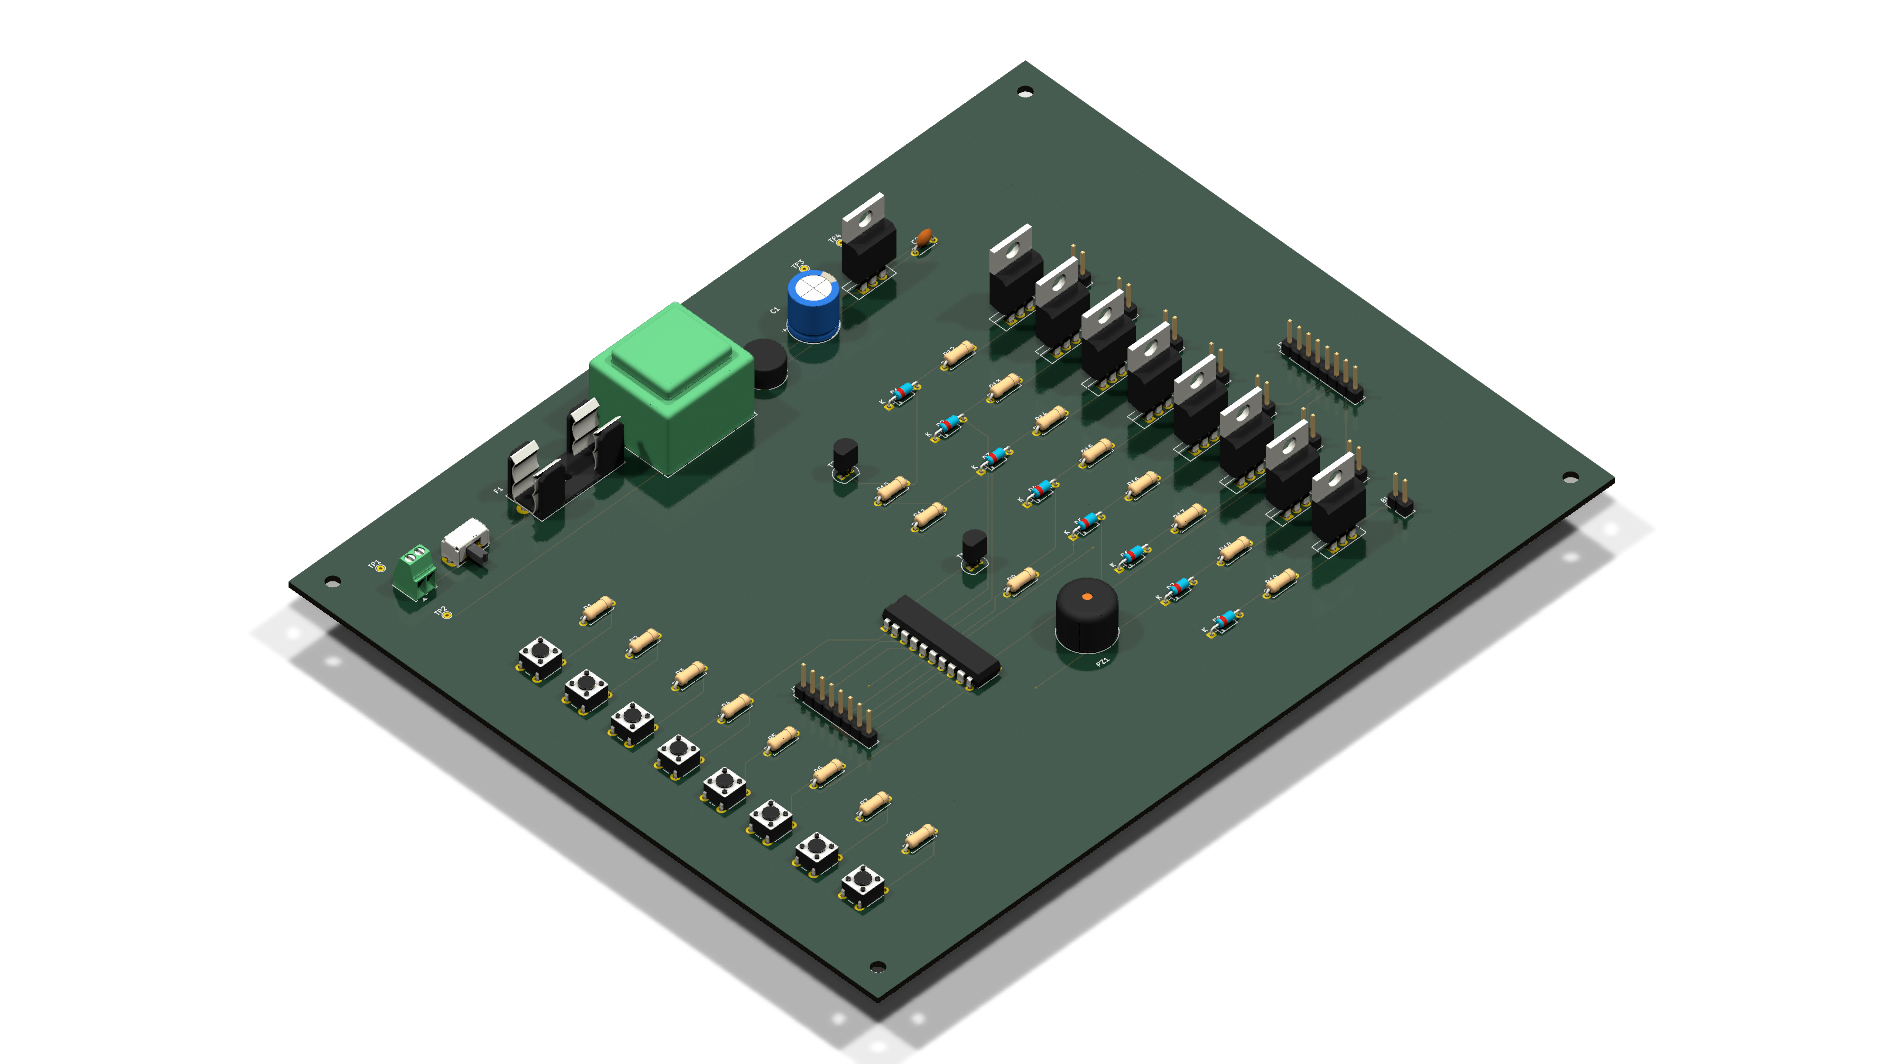
\includegraphics[width=0.98\textwidth]{3d_render_isometric.png}
    \caption{Photorealistic Raytraced 3D View of the Assembled Double-Layer Quiz Buzzer PCB.}
\end{figure}

\clearpage

% =========================================================================
% PAGE 3: SCHEMATIC SYNTHESIS & ERC VERIFICATION
% =========================================================================
\section{KiCad 9 Schematic Synthesis \& ERC Verification}

The complete schematic was synthesized with direct point-to-point wiring across all 73 components and 46 distinct electrical nets. Every symbol pin is explicitly connected through structured horizontal and vertical wiring stubs with dedicated net labels.

\subsection{Electrical Rules Check (ERC) Log}
\begin{verbatim}
ERC report (2026-11-11T15:37:58+0530, Encoding UTF8)
Report includes: Errors, Warnings, Exclusions

***** Sheet /

 ** ERC messages: 0  Errors 0  Warnings 0
[✓] ERC PASSED WITH ZERO VIOLATIONS!
\end{verbatim}

\begin{figure}[H]
    \centering
    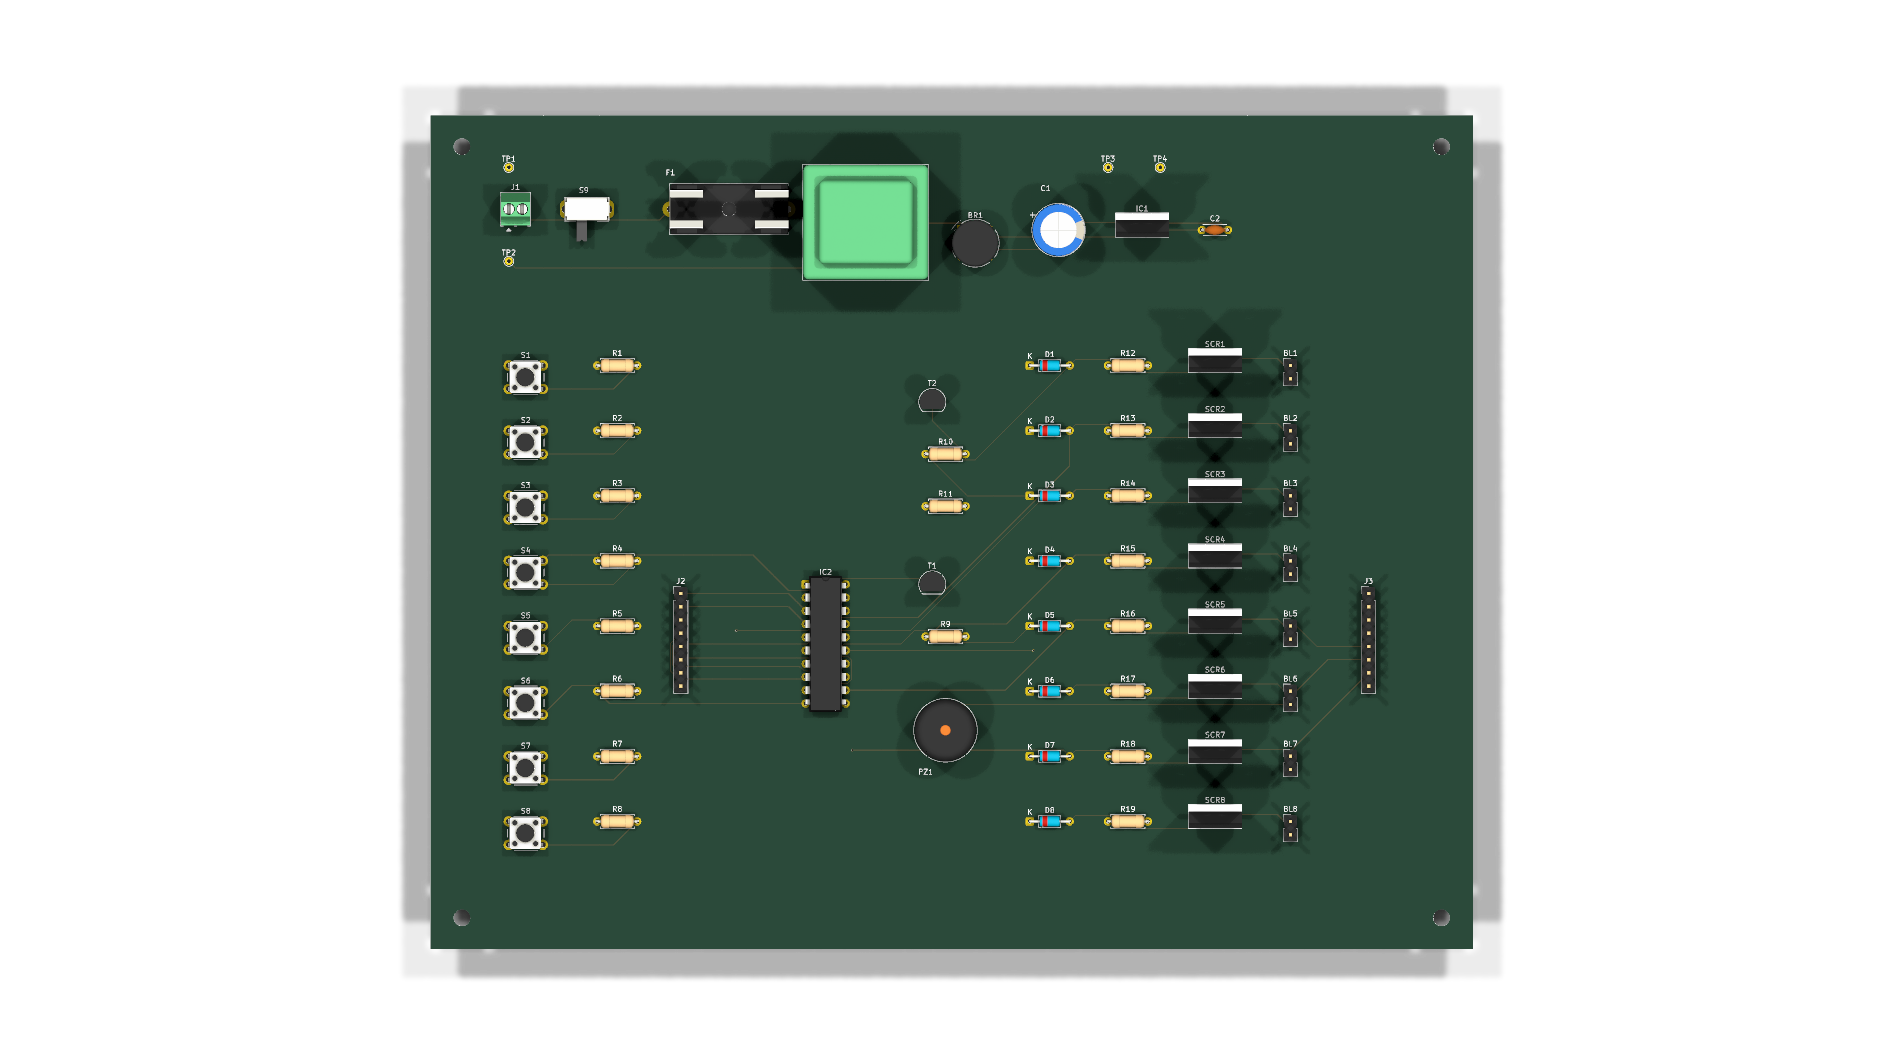
\includegraphics[width=0.95\textwidth]{3d_render_top.png}
    \caption{Orthogonal Top 3D View of the Manufactured Board Showing Functional Layout.}
\end{figure}

\clearpage

% =========================================================================
% PAGE 4: PCB LAYOUT, ROUTING & DRC VERIFICATION
% =========================================================================
\section{PCB Layout Architecture \& DRC Verification}

\subsection{Stackup and Physical Specifications}
\begin{itemize}
    \item \textbf{Layer 1 (F.Cu):} Point-to-point signal interconnects ($0.40\,\text{mm}$ trace width, $0.25\,\text{mm}$ clearance) and high-current power distribution traces ($0.80\,\text{mm}$ width).
    \item \textbf{Layer 2 (B.Cu):} Continuous solid Ground Plane ($\text{GND}$) poured over the entire board outline ($200 \times 160\,\text{mm}$) with thermal relief spokes on all through-hole component pads.
    \item \textbf{Physical Dimensions:} $200\,\text{mm} \times 160\,\text{mm}$ with 4 corner M3 mounting holes ($3.2\,\text{mm}$ drill diameter) with $5.0\,\text{mm}$ clearance borders.
\end{itemize}

\subsection{Design Rules Check (DRC) Report}
\begin{verbatim}
** DRC report for school_college_quiz_buzzer.kicad_pcb **
** Created on 2026-11-11T15:38:08+0530 **
** Report includes: Errors, Warnings **

** Found 0 DRC violations **

** Found 0 unconnected pads **

** Found 0 schematic parity issues **

** Found 0 Footprint errors **

** End of Report **
\end{verbatim}

\begin{figure}[H]
    \centering
    \begin{subfigure}[b]{0.48\textwidth}
        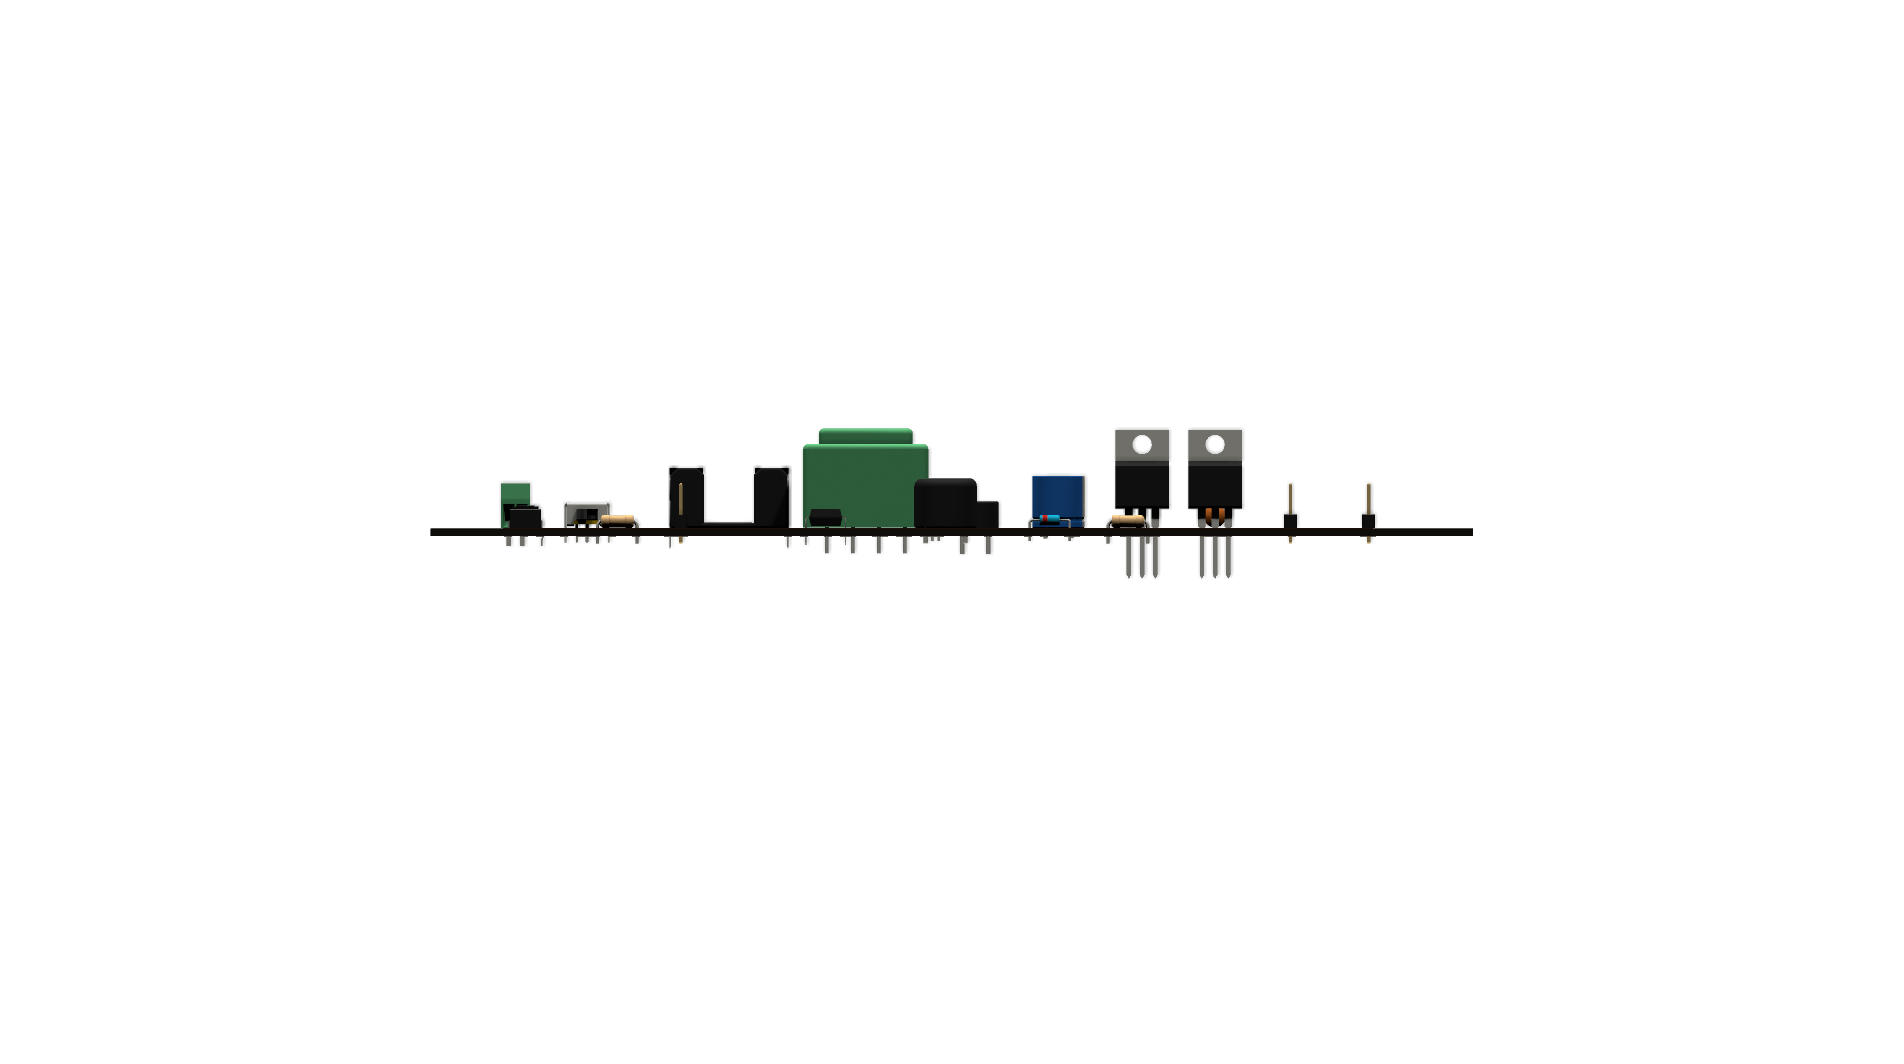
\includegraphics[width=\textwidth]{3d_render_front.png}
        \caption{Front Elevation View}
    \end{subfigure}
    \hfill
    \begin{subfigure}[b]{0.48\textwidth}
        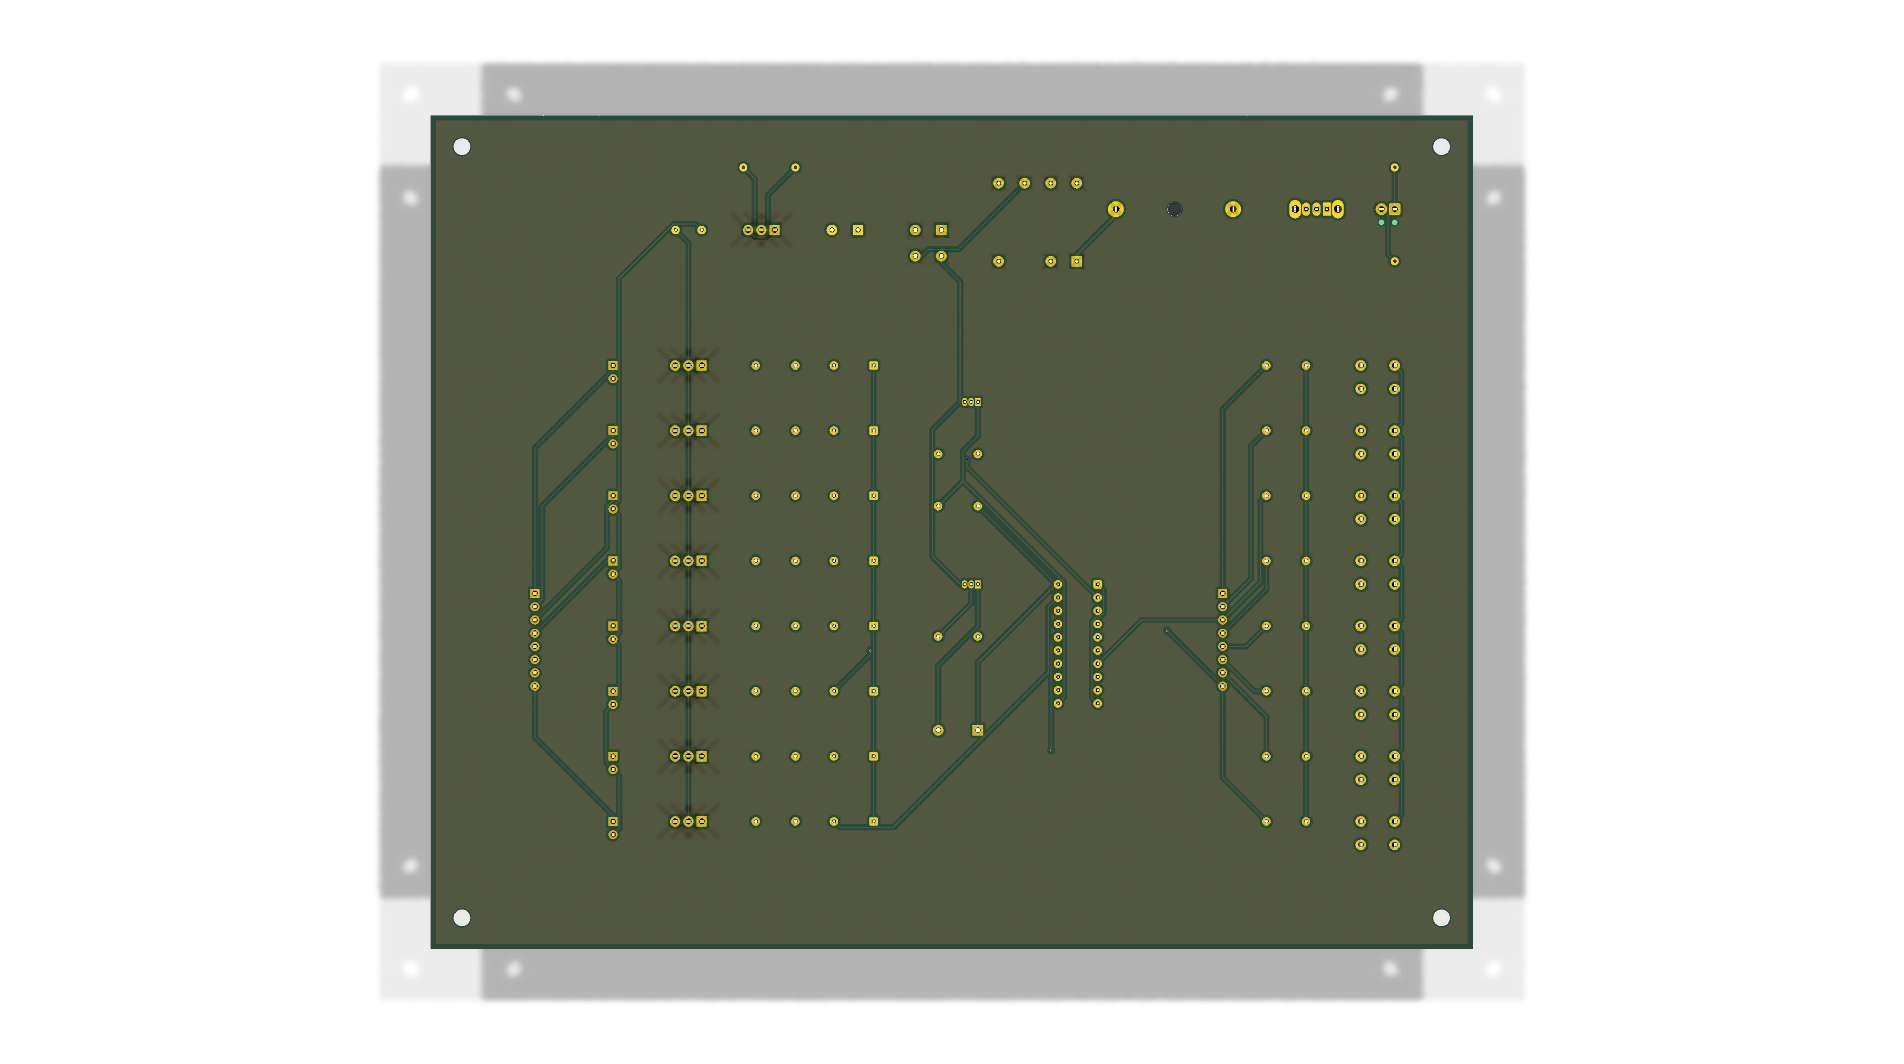
\includegraphics[width=\textwidth]{3d_render_bottom.png}
        \caption{Bottom Ground Plane View (B.Cu)}
    \end{subfigure}
    \caption{Raytraced Elevation and Solder Layer Views.}
\end{figure}

\clearpage

% =========================================================================
% PAGE 5: COMPLETE BILL OF MATERIALS (BOM)
% =========================================================================
\section{Complete Bill of Materials (BOM)}

\begin{table}[H]
\centering
\footnotesize
\renewcommand{\arraystretch}{1.2}
\begin{tabularx}{\textwidth}{l l l X l}
\toprule
\textbf{Item} & \textbf{Qty} & \textbf{Designators} & \textbf{Component Description} & \textbf{Package / Footprint} \\
\midrule
1 & 8 & BL1--BL8 & 6V Indicator Lamp / Remote Indicator Header & PinHeader\_1x02\_P2.54mm \\
2 & 1 & BR1 & 1A Bridge Rectifier, 100V & Diode\_Bridge\_Round\_D9.0mm \\
3 & 1 & C1 & 1000$\mu$F 25V Electrolytic Capacitor & CP\_Radial\_D10.0mm\_P5.00mm \\
4 & 1 & C2 & 0.1$\mu$F (100nF) 50V Ceramic Disc Capacitor & C\_Disc\_D4.3mm\_P5.00mm \\
5 & 8 & D1--D8 & 1N4148 Fast Switching Diodes & D\_DO-35\_SOD27\_P7.62mm \\
6 & 1 & F1 & 0.5A 250V Slow-Blow Cartridge Fuse & Fuseholder\_5x20mm\_Horizontal \\
7 & 4 & H1--H4 & M3 Chassis Mounting Holes & MountingHole\_3.2mm\_M3 \\
8 & 1 & IC1 & LM7805 5V Positive Linear Voltage Regulator & TO-220-3\_Vertical \\
9 & 1 & IC2 & 74LS373 Octal Transparent D-Type Latch & DIP-20\_W7.62mm \\
10 & 1 & J1 & 2-Pin Screw Terminal (AC 230V Mains Input) & TerminalBlock\_Phoenix\_2.54mm \\
11 & 1 & J2 & 8-Pin Remote Player Push Switch Header & PinHeader\_1x08\_P2.54mm \\
12 & 1 & J3 & 8-Pin Remote Lamp/Annunciator Header & PinHeader\_1x08\_P2.54mm \\
13 & 1 & PZ1 & 5V Continuous Tone Piezo Electric Buzzer & Buzzer\_12x9.5RM7.6 \\
14 & 8 & R1--R8 & 1.2k$\Omega$, 0.25W Metal Film Pull-Down Resistors & R\_Axial\_DIN0207\_P7.62mm \\
15 & 2 & R9, R10 & 1k$\Omega$, 0.25W Base Drive Resistors & R\_Axial\_DIN0207\_P7.62mm \\
16 & 1 & R11 & 56k$\Omega$, 0.25W Latch Enable Pull-Up Resistor & R\_Axial\_DIN0207\_P7.62mm \\
17 & 8 & R12--R19 & 1k$\Omega$, 0.25W SCR Gate Trigger Resistors & R\_Axial\_DIN0207\_P7.62mm \\
18 & 8 & S1--S8 & 6mm Tactile Push Button Switches (Player 1--8) & SW\_PUSH\_6mm \\
19 & 1 & S9 & SPDT Slide Switch (Mains Power ON/OFF) & SW\_Slide\_SPDT\_Angled \\
20 & 8 & SCR1--SCR8 & TYN612 Silicon Controlled Rectifiers (600V, 12A) & TO-220-3\_Vertical \\
21 & 2 & T1, T2 & BC548 NPN General Purpose BJT Transistors & TO-92\_Inline \\
22 & 4 & TP1--TP4 & Test Points (AC-L, AC-N, +5V, GND) & TestPoint\_THTPad\_D1.5mm \\
23 & 1 & X1 & Step-Down Transformer ($230\text{V} \to 7.5\text{V}$, 0.5VA) & Transformer\_Breve\_TEZ-22x24 \\
\bottomrule
\end{tabularx}
\caption{Complete Bill of Materials for the 8-Player Quiz Buzzer Board.}
\end{table}

\clearpage

% =========================================================================
% PAGE 6: VIVA VOCE QUESTIONS & PRACTICAL CONSIDERATIONS
% =========================================================================
\section{Viva Voce Design Considerations \& Practical Answers}

\begin{enumerate}
    \item \textbf{Why is a transparent latch (74LS373) preferred over edge-triggered flip-flops (74LS374) in this lockout circuit?}
    
    \textit{Answer:} The 74LS373 is level-sensitive ($\text{LE} = 1$ transparent, $\text{LE} = 0$ latched). This allows an instantaneous response to an asynchronous push button event. As soon as contestant $k$ presses switch $S_k$, output $Q_k$ immediately goes HIGH. Through the diode OR-ing bus, transistor $T_2$ is turned ON within nanoseconds, pulling $\text{LE}$ LOW ($0\,\text{V}$). This freezes all latch inputs before any competing switch signal can propagate, eliminating race conditions without requiring a master clock oscillator.

    \item \textbf{Why are SCRs utilized to drive the annunciator lamps instead of BJTs or MOSFETs?}
    
    \textit{Answer:} An SCR is a regenerative PNPN latching semiconductor. Once triggered by a brief gate pulse from $Q_k$ via $R_{12\dots 19}$, the SCR latches ON into continuous conduction and remains ON even after the contestant releases their push switch and the gate drive drops to zero. The lamp stays illuminated continuously until the master quiz master resets the system (cycling power switch $S_9$). A BJT or MOSFET would require continuous gate/base drive, turning OFF as soon as the switch is released.

    \item \textbf{What is the function of pull-down resistors $R_1$--$R_8$ ($1.2\,\text{k}\Omega$)?}
    
    \textit{Answer:} TTL logic inputs (like the 74LS series) float HIGH if left unconnected due to internal emitter pull-up structures. The $1.2\,\text{k}\Omega$ resistors sink the input leakage current ($I_{IL} \approx -0.4\,\text{mA}$) to ground, ensuring the voltage at $D_0$--$D_7$ remains well below the $V_{IL(\max)} = 0.8\,\text{V}$ threshold in the unpressed state.

    \item \textbf{Explain the design considerations for safety and isolation in the 230V AC mains section of the PCB.}
    
    \textit{Answer:} Under IPC-2221B standards, $230\,\text{V AC}$ ($325\,\text{V}_{\text{peak}}$) requires a minimum electrical creepage and clearance distance of $\ge 2.5\,\text{mm}$ (preferably $\ge 3.0\,\text{mm}$). The mains input block ($J_1$, $S_9$, $F_1$, and $X_1$ primary) is physically clustered in an isolated corner of the PCB, maintaining $>5.0\,\text{mm}$ isolation from low-voltage DC signals and the ground copper plane. Fuse $F_1$ ($0.5\,\text{A}$) provides rapid fault interruption against overcurrent and winding shorts.

    \item \textbf{What are the advantages of providing a continuous solid ground copper plane on the bottom layer (B.Cu)?}
    
    \textit{Answer:} A continuous ground plane provides:
    \begin{itemize}
        \item Minimal loop inductance and lowest possible impedance return path for high-frequency switching transients from the piezo buzzer and SCR gate firing.
        \item Excellent thermal spreading for the LM7805 regulator and SCRs.
        \item Effective EMI shielding against external noise interference in educational/auditorium environments.
    \end{itemize}
\end{enumerate}

\end{document}
